\chapter{Introduction}

% Human Perception of 3D Shapes https://link.springer.com/chapter/10.1007/978-3-540-74272-2_1
Shape perception is a long-standing and fundamental problem both in human
\cite{Pizlo:2007,Pizlo:2010}
and computer vision \cite{FurukawaHernandez:2015}.
In both disciplines, a large body of work focuses on 3D reconstruction, \eg
reconstructing objects or scenes from one or more views. 
The problem of reconstructing 3D scenes or objects is an inherently ill-posed
inverse problem because many configurations of shape, color, texture and
lighting may give rise to the very same views \cite{FurukawaHernandez:2015}.
In human vision, one of the fundamental problems is understanding
how the human visual system accomplishes such tasks; in computer vision,
in contrast, the goal is to develop 3D reconstruction systems.
Both disciplines are related through insights regarding the cues and constraints
used by humans to perceive 3D shapes. Results from human vision \cite{Pizlo:2007,Pizlo:2010}
suggest that these priors as well as the ability to process the provided cues
is innate and not learned. In computer vision, as well, cues and priors are commonly
built into 3D reconstruction pipelines through explicit assumptions.
Recently, however -- leveraging the success of deep learning -- researchers
started to learn shape models from data. Predominantly generative models have
been used to learn how to generate, manipulate and reason about shapes,
\eg \cite{GirdharGupta:2016,
DaiNiessner:2016,SharmaFritz:2016,BrockWeston:2016,
WuSongXiao:2015,WuTenenbaum:2016}. Learning such shape models
offers many interesting possibilities for a wide variety of problems
in 3D computer vision.

In this context, we focus on a specific problem in the realm of 3D reconstruction,
namely shape completion from point clouds, as
illustrated in Figure~\ref{fig:introduction}. This problem occurs when only a single view
of an individual object is provided and large parts of the object
are not observed or occluded. The problem is, however, also closely related to
surface reconstruction \cite{BergerSilva:2014} and, thus, has relevant applications
in computer graphics, as well. Motivated by the success of learning shape models,
we intend to tackle shape completion using a learning-based approach where
we make use of shape priors learned from large datasets of shapes
such as ModelNet \cite{WuSongXiao:2015} or ShapeNet \cite{ChangFunkhouserGuibasSavarese:2015}.
This idea, \ie learning-based shape completion, has recently gained traction
by works such as \cite{RieglerGeiger:2017,SmithMeger:2017,DaiNiessner:2016,
SharmaFritz:2016,FanSuGuibas:2016} or \cite{RezendeHeess:2016}.
Similarly, shape priors have already been
applied to many different problems in computer vision including 3D pose estimation
\cite{AdrianReid:2012,DambrevilleTannenbaum:2008,SandhuTannenbaum:2009,MenzeHeipkeGeiger:2015},
tracking \cite{MaSibley:2014,LeottaMundy:2009} or classical 3D reconstruction
\cite{GueneyGeiger:2015,DameReid:2013,BaoSavarese:2013}. In the case of shape completion,
however, most learning-based approaches still require full supervision; this means that
observations are either synthesized from known models, or datasets need to be annotated.
On real data, \eg on KITTI \cite{GeigerLenzUrtasun:2012,GeigerLenzStillerUrtasun:2013},
shape completion without supervision can be posed as energy minimization
problem over a latent space of shapes \cite{EngelmannStuecklerLeibe:2016,
BaoSavarese:2013,DameReid:2013}. In this case, shape completion usually
involves solving a complex minimization problem using iterative approaches.
Deep learning-based approaches, in contrast, can complete shapes using a single
forward pass of the learned network. We find
that both problems, the required supervision on the one hand and the computationally
expensive optimization problems at the other, constrain the applicability of
these approaches to real data considerably.

\begin{figure}[t]
  \centering
  %\begin{tikzpicture}
  %  \node at (1.5,1.75){Shape Set};
  %  \node[minimum width=6.25cm,minimum height=5.5cm,rectangle,draw=black] at (1.5,-1.25){};
  %  \node at (0,0) {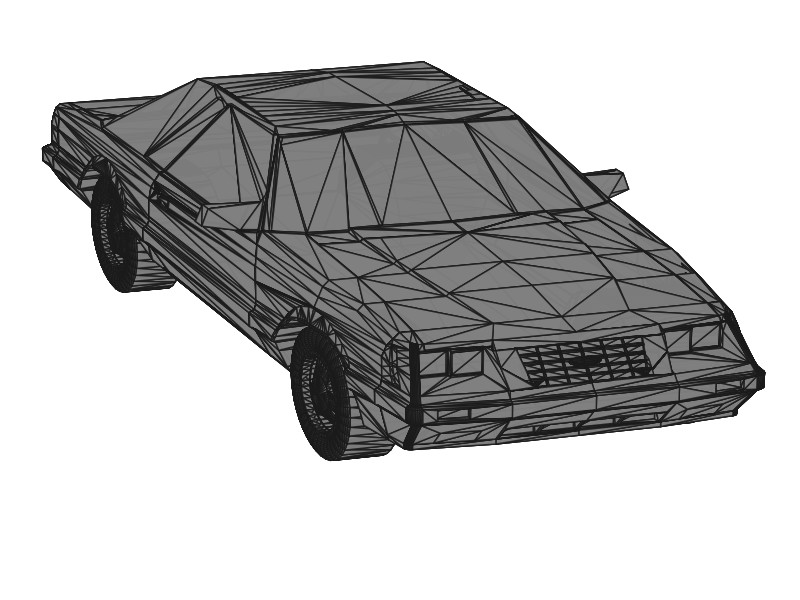
\includegraphics[width=3cm]{images/data/shapenet/simplification/1089cbe82dc0e72133d7c9e122eec9b6}};
  %  \node at (3,0) {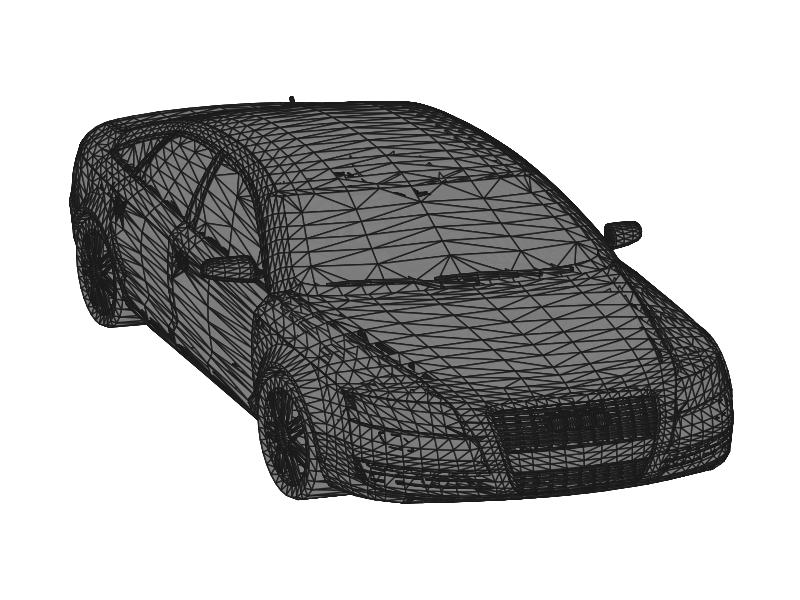
\includegraphics[width=3cm]{images/data/shapenet/simplification/1104f0924e03f2b6fc5886e868449015}};
  %  \node at (0,-2.5) {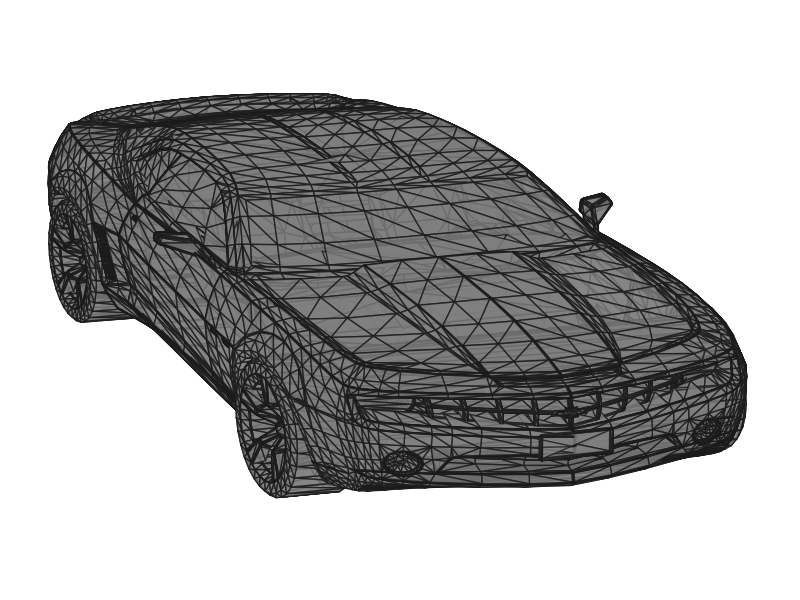
\includegraphics[width=3cm]{images/data/shapenet/simplification/1137cd58d6a45c6659a47b1880958de9}};
  %  \node at (3,-2.5) {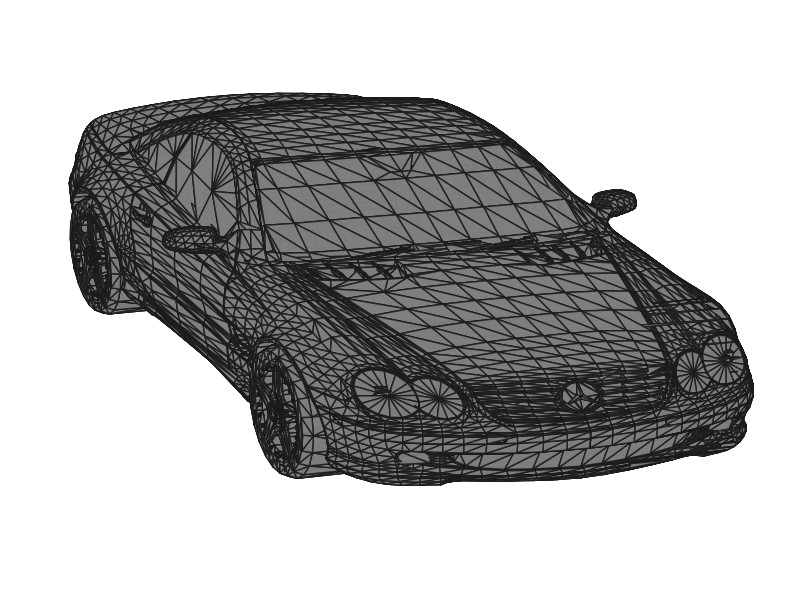
\includegraphics[width=3cm]{images/data/shapenet/simplification/119033fe083145e22f31600ac759c763}};
    
  %  \node at (8,1.75) {Observations};
  %  \node[rectangle,draw=black] at (8,0.15) {\includegraphics[width=5.5cm]{images/data/kitti/snapshot_01_rect}};
    
  %  \node[rectangle,draw=black,minimum height=2.5cm,minimum width=5.75cm,draw=black] at (8, -2.75) {};
  %  \node at (6.625, -2.75) {
  %    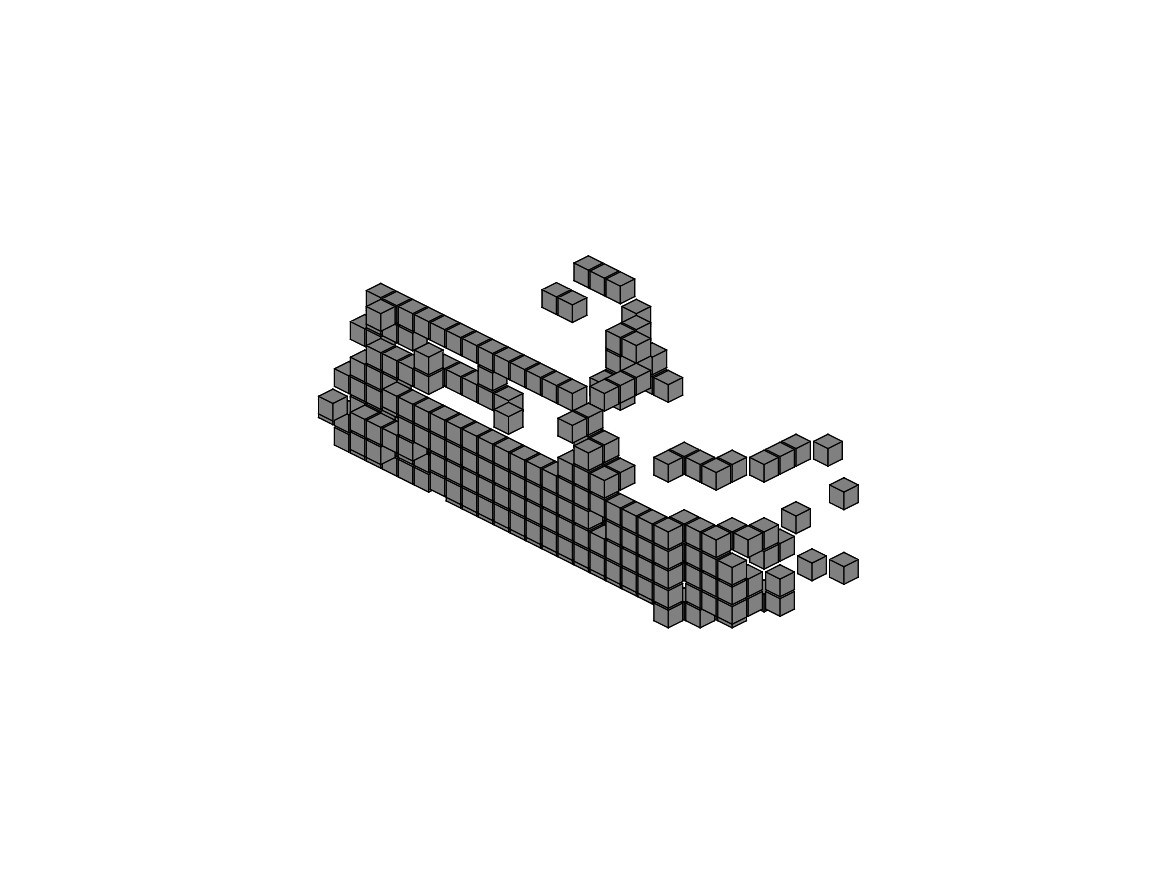
\includegraphics[width=2.75cm,trim={4.5cm 2.75cm 4.5cm 2.75cm},clip]{experiments/kitti/vae_occ_aml/15_long_statistics_combined/3_input_45}
  %  };    
  %  \node at (9.3725, -2.75) {
  %    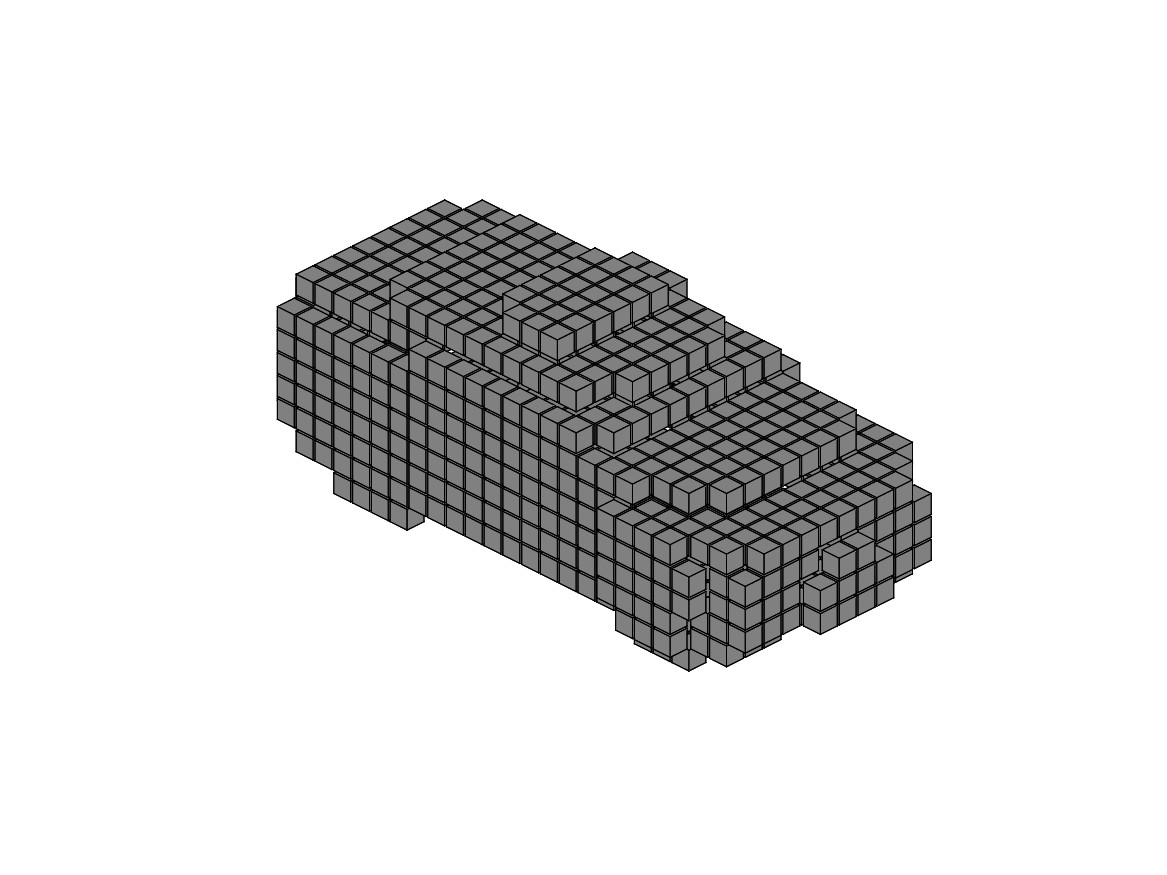
\includegraphics[width=2.75cm,trim={4.5cm 2.75cm 4.5cm 2.75cm},clip]{experiments/kitti/vae_occ_aml/15_long_statistics_combined/3_prediction_45}
  %  };
  %\end{tikzpicture}
  \vspace*{-1.25cm}
  \hspace*{-2cm}
  \begin{tikzpicture}
    \begin{scope}[on background layer]
      \node[rotate=45] at (-4,0.5) {
        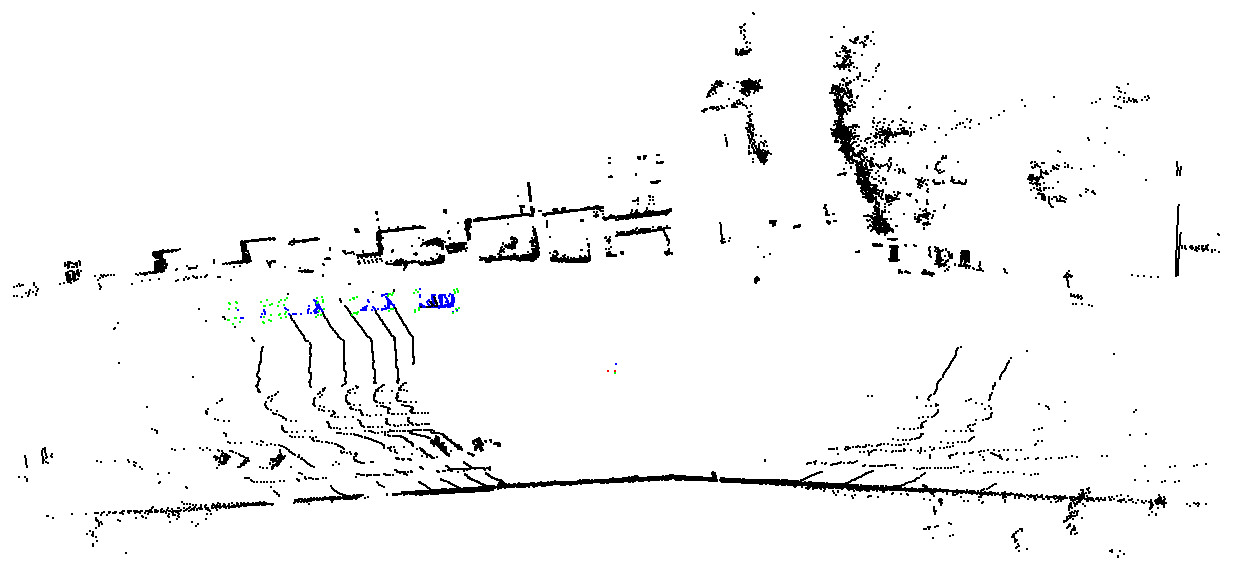
\includegraphics[width=8cm,trim={3cm 0 13cm 3cm},clip]{images/snapshot00_rect_fade}
      };
    \end{scope}
    
    \node[rectangle,draw=black,fill=white] at (3, 1.75) {
      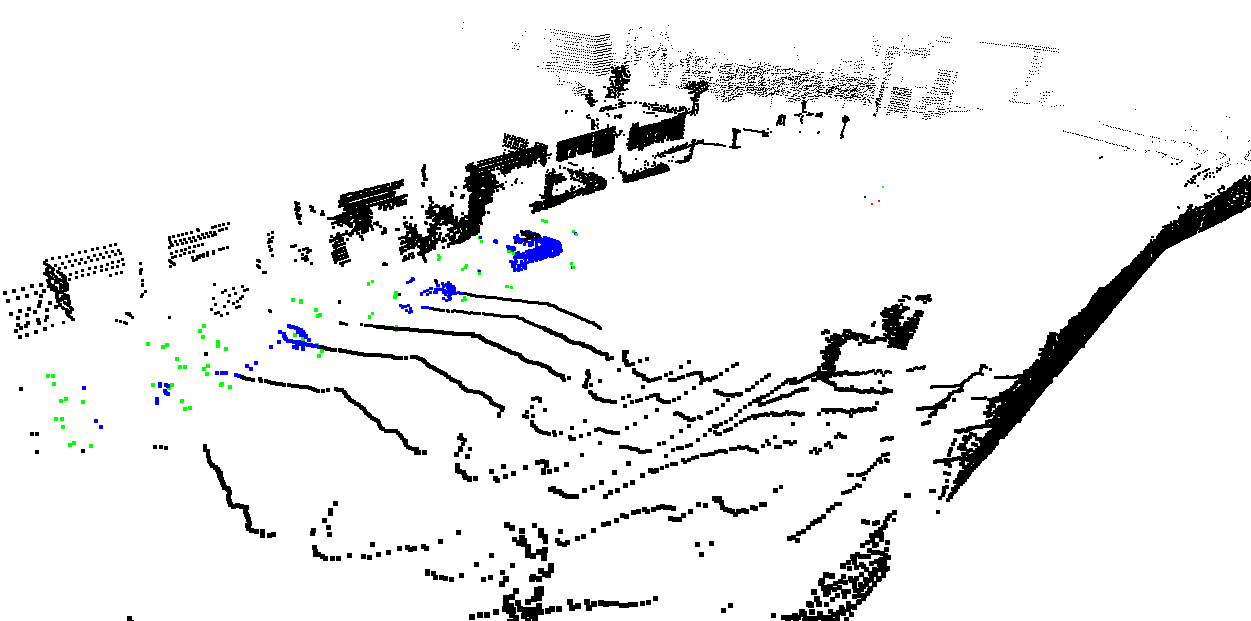
\includegraphics[width=8.85cm]{images/snapshot03_rect}
    };

    \node[rectangle,draw=black,fill=white] (input) at (0, -2) {
      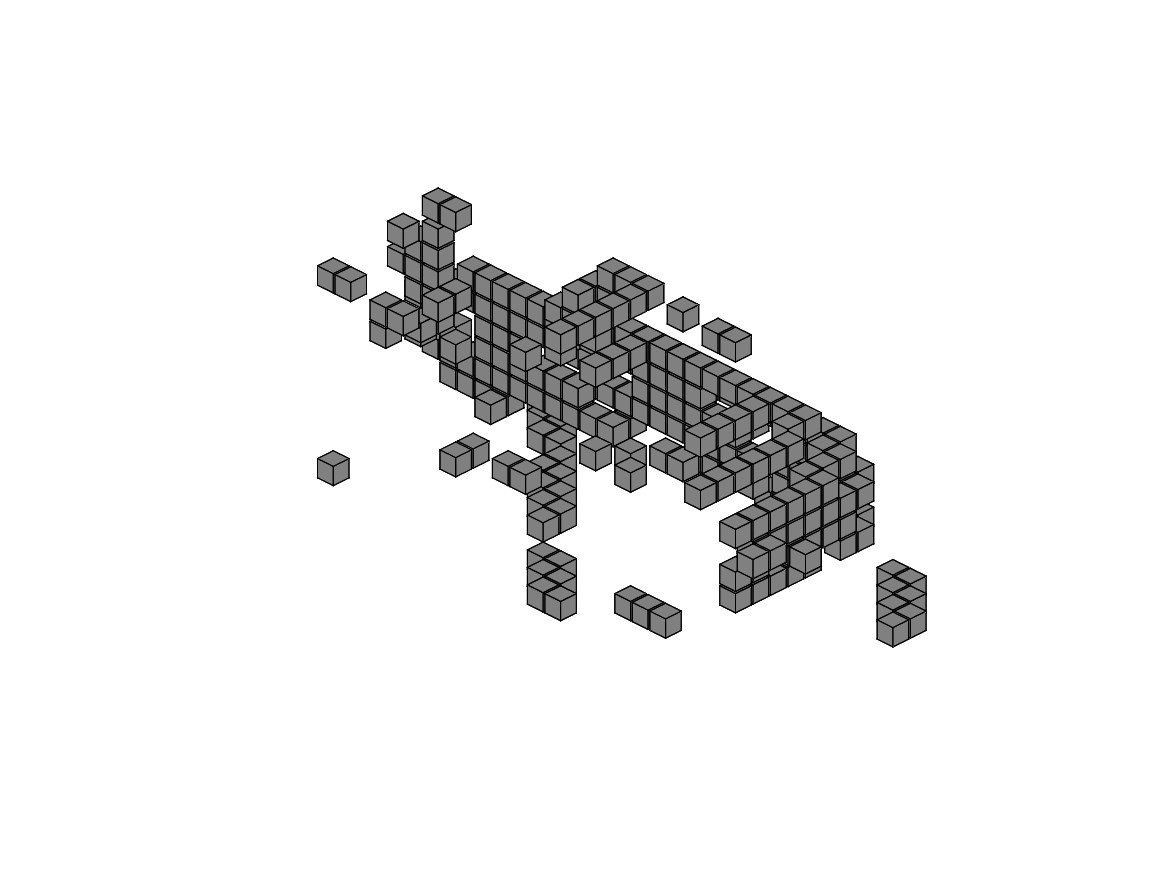
\includegraphics[height=2.25cm,trim={3cm 2cm 3cm 2cm},clip]{images/0_input_45}
    };
    \node at (0, -3.65) {\small Voxelized Observation};
    
    \node[rectangle,draw=black,fill=white] (output) at (6, -2) {
      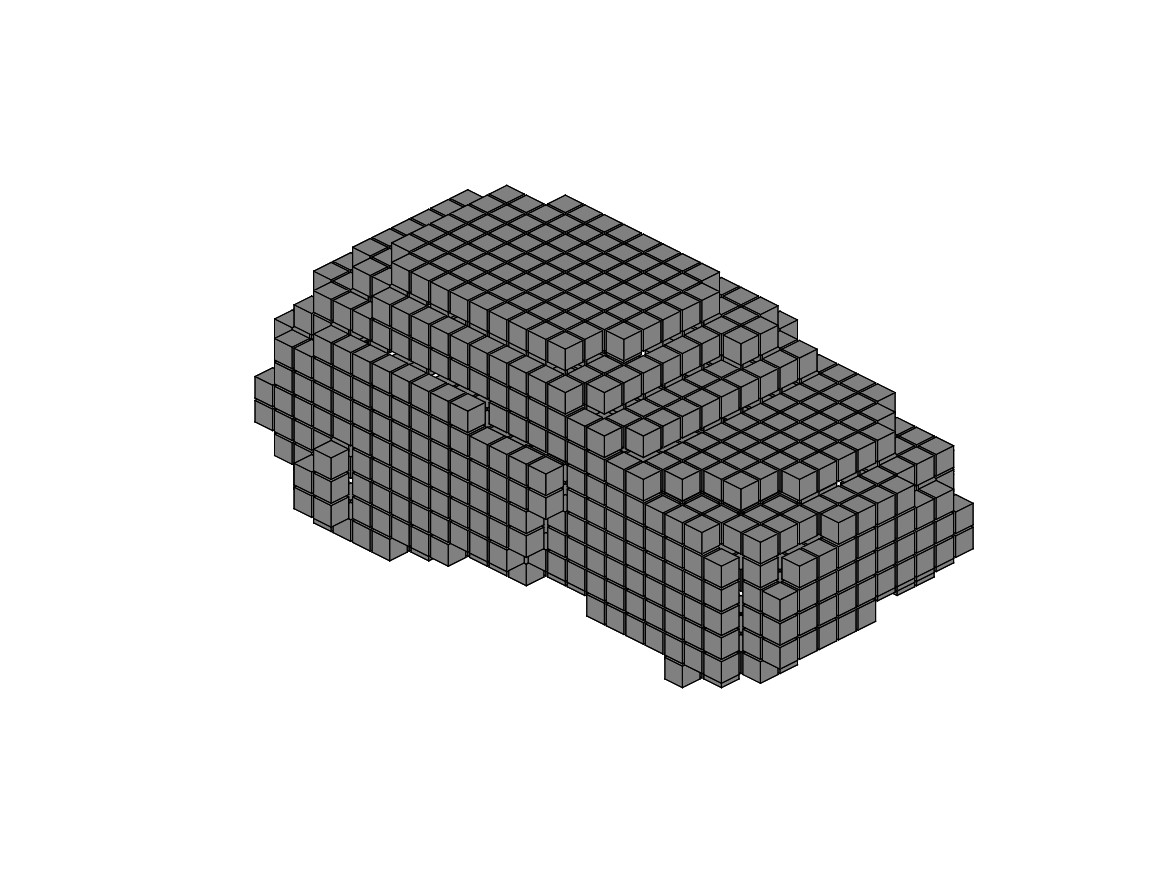
\includegraphics[height=2.25cm,trim={3cm 2cm 3cm 2cm},clip]{images/0_baseline_prediction_45}
    };
    \node at (6, -3.65) {\small Voxelized Shape};
    
    \draw[->] (input) -- (output);
    \node at (3, -1.4) {\small\begin{tabular}{c}Shape\\Completion\end{tabular}};
  \end{tikzpicture}
  \vspace{-0.5cm}
  
  % TODO short caption
  \caption{Illustration of the shape completion problem on
  KITTI \cite{GeigerLenzUrtasun:2012,GeigerLenzStillerUrtasun:2013} where we
  intend to learn shape completion of cars. We show a bird's eye view
  of a point cloud from KITTI in the background. On top, we show the same point cloud from
  a more natural viewpoint showing the points corresponding to cars
  in blue and the corresponding 3D bounding boxes, in particular their corners,
  highlighted in green. Below we show an illustration of the shape completion
  task. We extract point clouds of cars using the corresponding 3D bounding boxes
  and subsequently voxelize these points to obtain occupancy grids.
  Shape completion then describes the task of predicting a full shape which
  is also illustrated using occupancy grids, \ie in voxelized form.}
  \label{fig:introduction}
\end{figure}

In this thesis, we propose a probabilistic framework for shape completion
that tries to mitigate both problems: the need of annotated training data
%\cite{SmithMeger:2017,
%DaiNiessner:2016,SharmaFritz:2016,FanSuGuibas:2016,RezendeHeess:2016}
and the drawbacks of computationally involved optimization problems.
%\cite{EngelmannStuecklerLeibe:2016,BaoSavarese:2013,DameReid:2013}.
Following related work, \eg
\cite{SmithMeger:2017,GirdharGupta:2016,DaiNiessner:2016,
SharmaFritz:2016,BrockWeston:2016,WuSongXiao:2015} or \cite{WuTenenbaum:2016},
we utilize ShapeNet to learn
a strong shape prior using deep generative models, specifically variational
auto-encoders \cite{KingmaWelling:2013}. We hypothesize that using a strong
prior of possible shapes, we are able to learn how to complete shapes
under weak supervision, \ie only given knowledge about the object category
at hand. On real data, we additionally require knowledge about the object location
in the form of bounding boxes, \eg provided by an object detector.
By learning shape completion
using deep networks, we additionally reduce the problem to a forward pass
of the trained network.

\section{Contributions}

We propose two different probabilistic frameworks enabling us to learn
shape completion with weak supervision. In both cases, we first train
a shape prior, particularly a variational auto-encoder.
In the spirit of \cite{EngelmannStuecklerLeibe:2016}, we can then formulate
shape completion as maximum likelihood problem over the learned latent space.
Instead of maximizing the likelihood independently for distinct observations,
however, we follow the idea of amortized inference \cite{GershamGoodman:2014}
and learn to predict the maximum likelihood solution directly given the
corresponding observations. Specifically, we train an encoder,
which embeds the observations in the same latent space, using an unsupervised,
maximum likelihood loss between the observations and the corresponding shapes.
This variant of amortized maximum likelihood allows us to learn shape completion
under real conditions, \eg on KITTI,
and is able to compete with a fully-supervised baseline on a ShapeNet-based, synthetic dataset used for evaluation.

As alternative approach, we extend the general framework of latent space models,
as implemented by variational auto-encoders, to specifically account for the
observations. Applied to a pre-trained variational auto-encoder -- representing
the required shape prior -- we derive the evidence lower bound 
of this extended variational auto-encoder which we then
optimize in an unsupervised fashion, \ie only given the observations. We
also show that the underlying objective is closely related to
our amortized maximum likelihood approach. On our synthetic, ShapeNet-based dataset,
we experimentally demonstrate the applicability of the extended
variational auto-encoder regarding shape completion. Overall, we present two
approaches in favor of our claim that shape priors allow to learn shape completion
in an unsupervised fashion, thereby also introducing many interesting directions
for future research.

\section{Outline}

We formally introduce the problem of shape completion
under weak supervision in Chapter \ref{ch:problem}. Subsequently, Chapter
\ref{ch:related-work} reviews relevant related work. In Chapter \ref{ch:deep-learning},
we introduce the necessary background of training 3D convolutional neural networks.
We then discuss appropriate shape representations in Chapter 
\ref{ch:shape-representation}, before introducing the variational auto-encoder
which is used as shape prior. In Chapter \ref{ch:shape-inference},
we discuss how to use these models to learn shape completion with weak supervision.
The datasets used for our experiments are introduced in Chapter~\ref{ch:data}.
Finally, in Chapter \ref{ch:experiments},
we present experiments and conclude in Chapter \ref{ch:conclusion} including a
discussion of future work.
